\documentclass[aspectratio=43]{beamer}

% -------------------------------------------------
% Packages
% -------------------------------------------------
\usepackage[utf8]{inputenc}
\usepackage[T1]{fontenc}
\usepackage{lmodern}
\usepackage{amsmath,amssymb}
\usepackage{graphicx}
\usepackage{booktabs}
\usepackage{multicol}
\usepackage{tikz}
\usepackage{tkz-graph}
\usepackage{caption}
\usepackage{algorithm, algpseudocode}
\usepackage[french]{babel}
\usepackage{biblatex}


% -------------------------------------------------
% Theme configuration
% -------------------------------------------------
\usetheme{Madrid}
\usecolortheme{dolphin}

% -------------------------------------------------
% Custom colors
% -------------------------------------------------
\definecolor{mainblue}{RGB}{25,45,80}
\definecolor{lightblue}{RGB}{220,230,245}
\definecolor{darkgray}{RGB}{60,60,60}

\setbeamercolor{title}{fg=white,bg=mainblue}
\setbeamercolor{frametitle}{fg=white,bg=mainblue}
\setbeamercolor{structure}{fg=mainblue}
\setbeamercolor{section in head/foot}{bg=mainblue, fg=white}
\setbeamercolor{subsection in head/foot}{bg=lightblue, fg=black}
\setbeamercolor{author in head/foot}{bg=mainblue, fg=white}
\setbeamercolor{title in head/foot}{bg=mainblue, fg=white}
\setbeamercolor{date in head/foot}{bg=mainblue, fg=white}

% -------------------------------------------------
% Remove navigation symbols
% -------------------------------------------------
\setbeamertemplate{navigation symbols}{}

% -------------------------------------------------
% Footer
% -------------------------------------------------
\setbeamertemplate{footline}
{
    \leavevmode%
    \hbox{%
    \begin{beamercolorbox}[wd=.33\paperwidth,ht=2.5ex,dp=1ex,left]{author in head/foot}%
        \hspace{1em}\insertshortauthor
    \end{beamercolorbox}%
    
    \begin{beamercolorbox}[wd=.34\paperwidth,ht=2.5ex,dp=1ex,center]{title in head/foot}%
        \insertshorttitle
    \end{beamercolorbox}%
    
    \begin{beamercolorbox}[wd=.33\paperwidth,ht=2.5ex,dp=1ex,right]{date in head/foot}%
        \insertframenumber{} / \inserttotalframenumber
        \hspace{1em}
    \end{beamercolorbox}}%
    
    \vskip0pt%
}

% -------------------------------------------------
% Title page information
% -------------------------------------------------
\title[b-couplages stables]{Implémenter un réseau pair à pair à l'aide des couplages}
\author[Simon Roux]{Simon Roux}
\institute{
    TIPE - MPI
}
\date{\today}

% -------------------------------------------------
% Table of contents at beginning of sections
% -------------------------------------------------
\AtBeginSection[]
{
    \begin{frame}
        \frametitle{Sommaire}
        \tableofcontents[currentsection]
    \end{frame}
}

% -------------------------------------------------
% Document
% -------------------------------------------------
\begin{document}

% -------------------------------------------------
% Title slide
% -------------------------------------------------
\begin{frame}
    \titlepage
\end{frame}

% =================================================
\begin{frame}
\frametitle{Introduction - Partage d'un fichier F dans un réseau}
\begin{columns}
\column{0.5\textwidth}
\centering
    \begin{figure}
    \begin{tikzpicture}
        \SetUpEdge[lw = 1.5pt,
        color = orange,
        labelcolor = white]
        \GraphInit[vstyle=Normal] \SetGraphUnit{3}
        \tikzset{VertexStyle/.append style={fill = red!50}}
        \Vertex{Serv}
        \Vertex[x=0, y=-2]{A}
        \Vertex[x=0, y=2]{C}
        \Vertex[x=-2, y=0]{B}
        \Vertex[x=2, y=0]{D}
        \Edge[label=F](Serv)(A)
        \Edge[label=F](Serv)(B)
        \Edge[label=F](Serv)(C)
        \Edge[label=F](Serv)(D)
    \end{tikzpicture}
    \caption{Partage d'un fichier par un serveur}
    \end{figure}

\column{0.5\textwidth}

\begin{figure}
\begin{tikzpicture}
    \centering
        \SetUpEdge[lw = 1.5pt,
        color = red,
        labelcolor = white]
        \GraphInit[vstyle=Normal] \SetGraphUnit{3}
        \tikzset{VertexStyle/.append style={fill = red!50}}
        \Vertex{A}
        \node[anchor=east] at (A.west) {[F]};
        \Vertex[x=0, y=4]{B}
        \Vertex[x=4, y=0]{E}
        \Vertex[x=4, y=4]{D}
        \Vertex[x=2, y=2]{C}
        \node[anchor=east] at (C.west) {[F]};
        \tikzset{EdgeStyle/.style={->}}
        \Edge[label=F](A)(B)
        \Edge[label=F](A)(E)
        \Edge[label=F](C)(D)
        \tikzset{EdgeStyle/.style={color=orange, ->}}
        \Edge[label=F](A)(C)
    \end{tikzpicture}
    \caption{Partage d'un fichier dans un réseau P2P}
    \vspace{1cm}
    \end{figure}
\end{columns}
\end{frame}


\begin{frame}
    \frametitle{Définition 1 - Réseau}
    \centering
    \begin{tikzpicture}
        \SetUpEdge[lw = 1.5pt,
        color = orange,
        labelcolor = white]
        \GraphInit[vstyle=Normal] \SetGraphUnit{3}
        \tikzset{VertexStyle/.append style={fill = red!50}}
        \Vertex{A}
        \Vertex[x=0, y=4]{B}
        \Vertex[x=4, y=0]{E}
        \Vertex[x=4, y=4]{D}
        \Vertex[x=2, y=2]{C}
    \end{tikzpicture}

    \vspace{1cm}
    \textbf{Réseau:} Ensemble d'utilisateurs (=noeuds)
\end{frame}


\begin{frame}
\frametitle{Définition 2 - b-couplage}
\begin{columns}
\column{0.5\textwidth}
\centering
\begin{figure}
\begin{tikzpicture}
        \SetUpEdge[lw = 1.5pt,
        color = red,
        labelcolor = white]
        \GraphInit[vstyle=Normal] \SetGraphUnit{3}
        \tikzset{VertexStyle/.append style={fill = red!50}}
        \Vertex{A}
        \Vertex[x=0, y=4]{B}
        \Vertex[x=4, y=0]{E}
        \Vertex[x=4, y=4]{D}
        \Vertex[x=2, y=2]{C}
        \tikzset{EdgeStyle/.style={-}}
        \Edge(B)(C)
        \Edge(D)(E)
    \end{tikzpicture}
    \caption{Cas $b=1$}
    \end{figure}

\column{0.5\textwidth}
\centering
\begin{figure}
\begin{tikzpicture}
        \SetUpEdge[lw = 1.5pt,
        color = red,
        labelcolor = white]
        \GraphInit[vstyle=Normal] \SetGraphUnit{3}
        \tikzset{VertexStyle/.append style={fill = red!50}}
        \Vertex{A}
        \Vertex[x=0, y=4]{B}
        \Vertex[x=4, y=0]{E}
        \Vertex[x=4, y=4]{D}
        \Vertex[x=2, y=2]{C}
        \tikzset{EdgeStyle/.style={-}}
        \Edge(A)(B)
        \Edge(B)(C)
        \Edge(C)(D)
        \Edge(D)(E)
        \Edge(E)(A)
    \end{tikzpicture}
    \caption{Cas $b=2$}
    \end{figure}
    \end{columns}

    \vspace{1cm}
    \textbf{$b$-couplage:} $C$ ensemble d'arêtes vérifiant $\forall n\in N, \space \sharp\{\{n, p\}\space  | \space p \in N\} \space \leq \space b$.
\end{frame}


\begin{frame}
    \frametitle{Définition 3 - Listes de préférences}
\centering
\begin{tikzpicture}
        \SetUpEdge[lw = 1.5pt,
        color = orange,
        labelcolor = white]
        \GraphInit[vstyle=Normal] \SetGraphUnit{3}
        \tikzset{VertexStyle/.append style={fill = red!50}}
        \Vertex{A}
        \node[anchor=east] at (A.west) {[C; D; B; E]};
        \Vertex[x=0, y=4]{B}
        \Vertex[x=4, y=0]{E}
        \Vertex[x=4, y=4]{D}
        \Vertex[x=2, y=2]{C}
        \node[anchor=east] at (B.west) {[C; A; E; D]};
        \node[anchor=east] at (C.west) {[B; E; D; A]};
        \node[anchor=west] at (D.east) {[C; E; A; B]};
        \node[anchor=west] at (E.east) {[D; C; A; B]};
    \end{tikzpicture}
    
    \vspace{0.2cm}
    La \textit{liste de préférences} d'un noeud ordonne les autres noeuds
\end{frame}


\begin{frame}
    \frametitle{Définition 4 - Graphe de préférences}
    \centering
    \begin{tikzpicture}
        \SetUpEdge[lw = 1.5pt,
        color = orange,
        labelcolor = white]
        \GraphInit[vstyle=Normal] \SetGraphUnit{3}
        \tikzset{VertexStyle/.append style={fill = red!50}}
        \Vertex{A}
        \node[anchor=east] at (A.west) {[C; D; B; E]};
        \Vertex[x=0, y=4]{B}
        \Vertex[x=4, y=0]{E}
        \Vertex[x=4, y=4]{D}
        \Vertex[x=2, y=2]{C}
        \node[anchor=east] at (B.west) {[C; A; E; D]};
        \node[anchor=east] at (C.west) {[B; E; D; A]};
        \node[anchor=west] at (D.east) {[E; C; A; B]};
        \node[anchor=west] at (E.east) {[C; D; A; B]};
        \tikzset{EdgeStyle/.style={->}}
        \Edge(A)(C)
        \Edge(B)(C)
        \Edge(D)(E)
        \Edge(E)(C)
        \tikzset{EdgeStyle/.style={bend right, ->}}
        \Edge(C)(B)
    \end{tikzpicture}

    \vspace{1cm}
    \textbf{Graphe de préférences:} Sommets = utilisateurs, Arête de $X$ à $Y$ si $Y$ est premier dans la liste de préférence de $X$
    \textbf{Graphe cyclique:} s'il y a un $k$-cycle pour $k\ge2$
\end{frame}



\begin{frame}
\frametitle{Définition 5 - b-couplage stable}
\begin{columns}
\column{0.5\textwidth}
\begin{figure}
\begin{tikzpicture}
        \SetUpEdge[lw = 1.5pt,
        color = red,
        labelcolor = white]
        \GraphInit[vstyle=Normal] \SetGraphUnit{3}
        \tikzset{VertexStyle/.append style={fill = red!50}}
        \Vertex{A}
        \Vertex[x=4, y=0]{B}
        \Vertex[x=2, y=2]{C}
        \tikzset{EdgeStyle/.style={-}}
        \Edge(A)(B)
        \tikzset{EdgeStyle/.style={dotted, color=black}}
        \Edge(A)(C)
        \Edge(C)(B)
        \node[anchor=north] at (B.south) {[A; C]};
        \node[anchor=south] at (C.north) {[A; B]};
        \node[anchor=north] at (A.south) {[C; B]};
    \end{tikzpicture}
    \caption{Couplage non stable}
    \end{figure}

\column{0.5\textwidth}
\begin{figure}
\begin{tikzpicture}
        \SetUpEdge[lw = 1.5pt,
        color = red,
        labelcolor = white]
        \GraphInit[vstyle=Normal] \SetGraphUnit{3}
        \tikzset{VertexStyle/.append style={fill = red!50}}
        \Vertex{A}
        \Vertex[x=4, y=0]{B}
        \Vertex[x=2, y=2]{C}
        \tikzset{EdgeStyle/.style={-}}
        \Edge(A)(B)
        \tikzset{EdgeStyle/.style={dotted, color=black}}
        \Edge(A)(C)
        \Edge(C)(B)
        \node[anchor=north] at (B.south) {[A; C]};
        \node[anchor=south] at (C.north) {[A; B]};
        \node[anchor=north] at (A.south) {[B; C]};
    \end{tikzpicture}
    \caption{Couplage stable}
    \end{figure}
\end{columns}
 
    \vspace{1cm}
    \textbf{$R_n(p)$:} Rang du noeud p dans la liste de préférence de n.
    \vspace{0.2cm}
    \textbf{$b$-couplage stable:} Couplage $C$ de cardinal maximal vérifiant $\forall \{n, p\}\in C, \forall \{n', p'\} \in N^{2}, R_n(p) > R_n(p')$ ou $R_p(n) > R_p(n')$.
\end{frame}



\begin{frame}
\frametitle{Pertinence les b-couplages stables}
    \begin{itemize}
        \item Optimiser\footnote{Au sens des listes de préférences} les transferts de fichiers = déterminer un b-couplage stable
        \item Pourquoi les b-couplages stables?
        \begin{itemize}
            \item Donne le même rôle à tous les noeuds
            \item Choix effectués localement par les noeuds
        \end{itemize}
    \end{itemize}
\end{frame}




% =================================================

\begin{frame}
    \frametitle{Méthodologie}

    \begin{block}{Proposition}
    Soit $b\in \mathbb{N}$ et $R$ un réseau. Si le graphe de préférence de $R$ est acyclique, alors $R$ admet un $b$-couplage stable.
    \end{block}

    Dans un graphe de préférence acyclique:
    \begin{itemize}
        \item Implémentation pour un réseau statique
        \item Première adaptation pour un réseau dynamique
        \item Deuxième adaptation moins naïve pour un réseau dynamique
    \end{itemize}
    \vspace{0.3cm}

    puis adaptation dans un graphe de préférence cyclique:

\end{frame}



% =================================================

\begin{frame}
    \frametitle{Calcul de couplage stable statique}
        Soit $n$, $p$ deux utilisateurs

        \begin{block}{Définition}
        La paire $\{n, p\}$ est bloquante si $n$ ou $p$ n'est pas complètement couplé, ou si $n$ et $p$ préfèreraient être couplés ensemble.
        \end{block}
        
        \begin{figure}
            \centering
            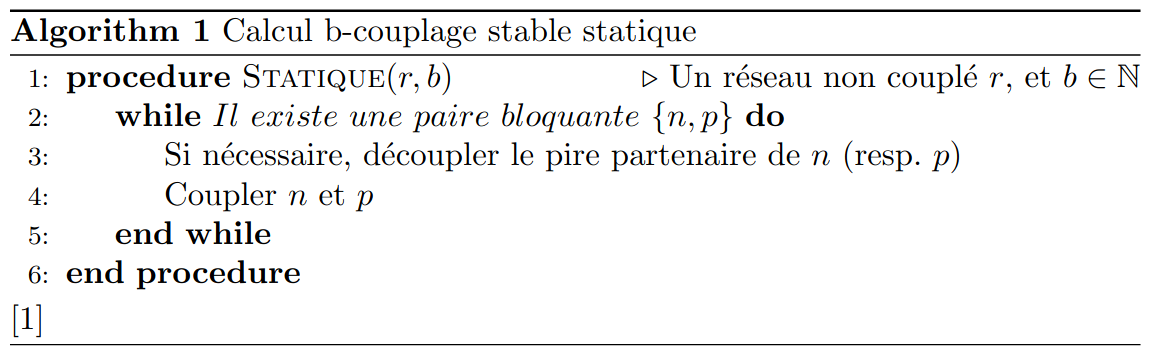
\includegraphics[width=0.8\linewidth]{algo1.png}
        \end{figure}
\end{frame}


\begin{frame}
    \frametitle{Couplage stable statique - Résultats}
        \begin{figure}
            \centering
            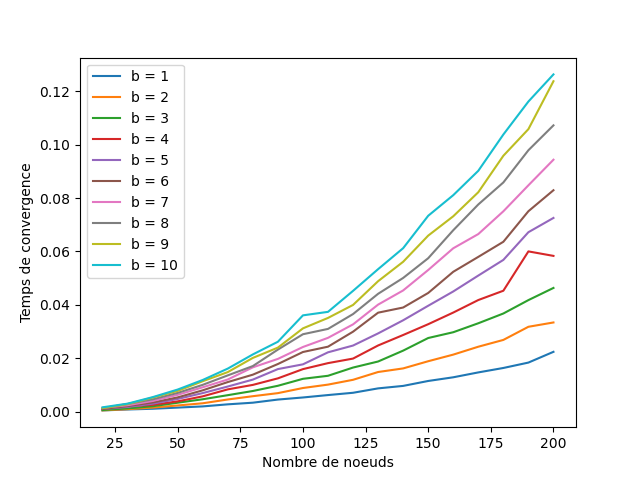
\includegraphics[width=0.7\linewidth]{chart_fab_p=1.png}
            \caption{Temps de convergence de $STATIQUE$}
        \end{figure}
\end{frame}

\begin{frame}
    \frametitle{Couplage stable statique - Résultats}
        \begin{figure}
            \centering
            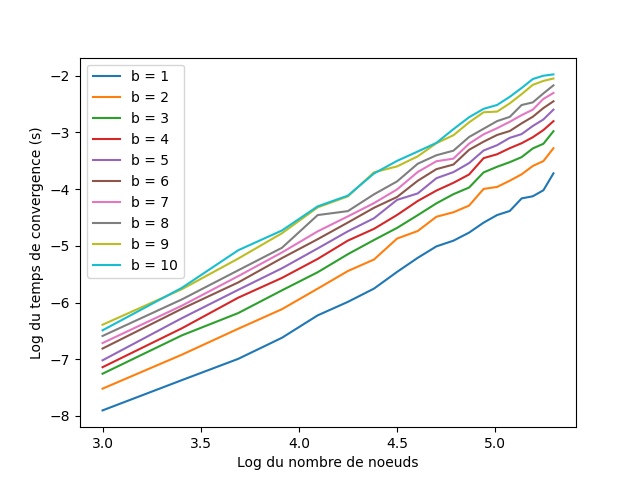
\includegraphics[width=0.7\linewidth]{chart_fab_log.png}
            \caption{Logarithme du temps de convergence de $STATIQUE$}
        \end{figure}
    Attendu: $O(2^{n+b})$
\end{frame}


% =================================================

\begin{frame}
    \frametitle{Couplage stable dynamique naïf}
    Description de l'algorithme:
    \begin{itemize}
        \item Construction d'un b-couplage stable
        \item A chaque modification, calcul d'un nouveau b-couplage stable via $STATIQUE$
    \end{itemize}
\end{frame}

\begin{frame}
    \frametitle{Couplage stable dynamique naïf - Résultats}
        \begin{figure}
            \centering
            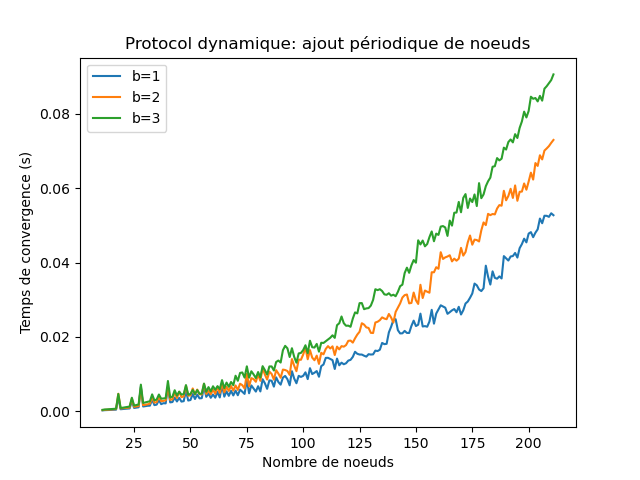
\includegraphics[width=0.7\linewidth]{chart_dyna_t.png}
            \caption{Ajout successifs de 180 noeuds à partir de $|R|=10$}
        \end{figure}
\end{frame}



% =================================================

\begin{frame}
    \frametitle{Calcul de couplage stable dynamique par modification locale}
    Description de l'algorithme:
    \begin{itemize}
        \item Construit d'un b-couplage stable
        \item A chaque modification, changement local du couplage autour de la modification
    \end{itemize}
    Mesure de satisfaction\footnote{\textit{G. Georgiadis, M. Papatriantafilou}} pour un noeud $i$:
        \begin{equation}
            S_i = \frac{c_i}{b} + \sum_{j}{\frac{R_j - C_j}{L_j b} \in [0, 1]}
        \end{equation}
    Intuitivement, elle quantifierait la stabilité du couplage.
\end{frame}

\begin{frame}
    \frametitle{Méthode de modification locale - Mesure de satisfaction}   
    \begin{figure}
        \centering
        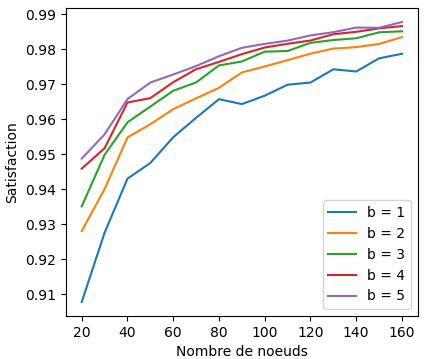
\includegraphics[width=0.7\linewidth]{chart_fab_sat.png}
        \caption{Satisfaction d'un couplage obtenu de $STATIQUE$}
    \end{figure}
\end{frame}

\begin{frame}
    \frametitle{Méthode de modification locale - Résultats}
    \begin{figure}
        \centering
        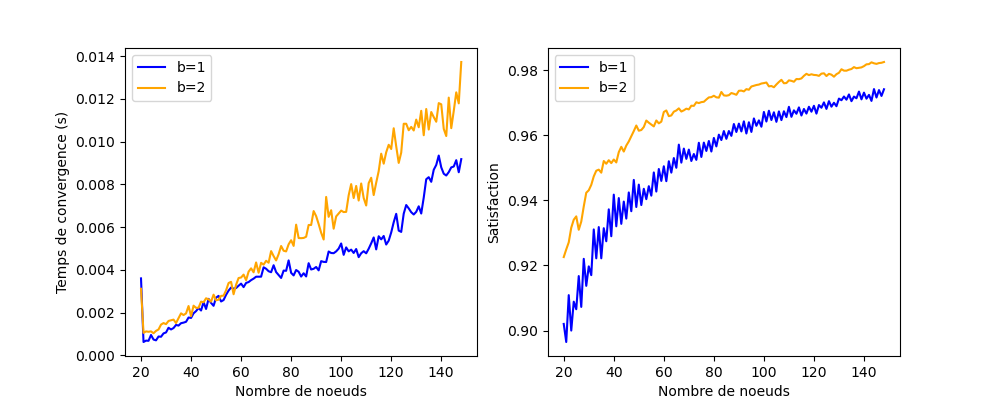
\includegraphics[width=0.9\linewidth]{chart_adap_add.png}
        \caption{Ajout successifs de 180 noeuds à partir de $|R|=20$}
    \end{figure}
\end{frame}

\begin{frame}
    \frametitle{Méthode de modification locale - Résultats}
    \begin{figure}
        \centering
        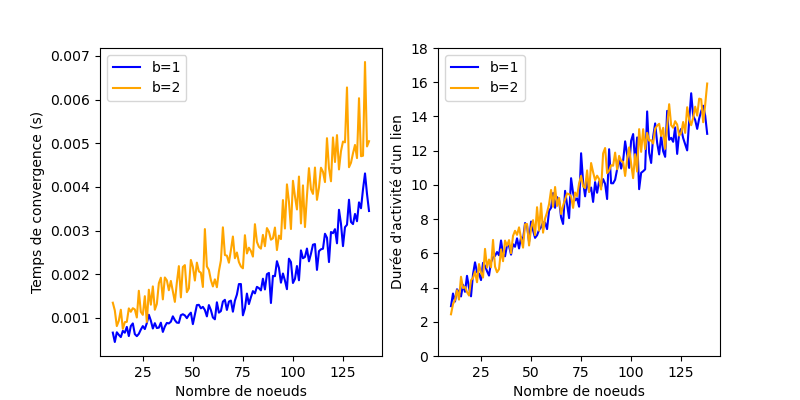
\includegraphics[width=0.8\linewidth]{chart_adap_t_span.png}
        \caption{Ajout et retrait successifs à $|R|$ fixé}
    \end{figure}
\end{frame}


% =================================================

\begin{frame}
    \frametitle{S'affranchir de la condition d'acyclicité}
    Le graphe de préférence est désormais cyclique

    Description de l'algorithme:
    \begin{itemize}
        \item On retient les paires bloquantes parcourues
        \item Si on détecte un cycle, suppression d'un arête du cycle
        \item Si un noeud n'a plus d'arêtes, il est supprimé
    \end{itemize}
\end{frame}

\begin{frame}
    \frametitle{S'affranchir de la condition d'acyclicité - Exemple}
    \centering
    \begin{tikzpicture}
        \SetUpEdge[lw = 1.5pt,
        color = orange,
        labelcolor = white]
        \GraphInit[vstyle=Normal] \SetGraphUnit{3}
        \tikzset{VertexStyle/.append style={fill = red!50}}
        \Vertex{A}
        \node[anchor=east] at (A.west) {[B; C]};
        \Vertex[x=0, y=4]{B}
        \Vertex[x=2, y=2]{C}
        \node[anchor=east] at (B.west) {[C; A]};
        \node[anchor=west] at (C.north) {[A; B]};
        \tikzstyle{EdgeStyle}=[color=red, ->]
        \Edge(A)(B)
        \Edge(B)(C)
        \Edge(C)(A)
    \end{tikzpicture}
\end{frame}



\begin{frame}
    \frametitle{S'affranchir de la condition d'acyclicité - Exemple}
    \centering
    \begin{tikzpicture}
        \SetUpEdge[lw = 1.5pt,
        color = orange,
        labelcolor = white]
        \GraphInit[vstyle=Normal] \SetGraphUnit{3}
        \tikzset{VertexStyle/.append style={fill = red!50}}
        \Vertex{A}
        \node[anchor=east] at (A.west) {[B; D; C; E]};
        \Vertex[x=0, y=4]{B}
        \Vertex[x=4, y=0]{E}
        \Vertex[x=4, y=4]{D}
        \Vertex[x=2, y=2]{C}
        \node[anchor=east] at (B.west) {[C; A; E; D]};
        \node[anchor=west] at (C.north) {[A; D; E; B]};
        \node[anchor=west] at (D.east) {[C; E; A; B]};
        \node[anchor=west] at (E.east) {[C; D; A; B]};
        \tikzset{EdgeStyle/.style={->}}
        \Edge(E)(C)
        \tikzstyle{EdgeStyle}=[color=red, ->]
        \Edge(A)(B)
        \Edge(B)(C)
        \Edge(C)(A)
        \tikzstyle{EdgeStyle}=[bend left, color=orange, ->]
        \Edge(D)(E)
    \end{tikzpicture}
\end{frame}

\begin{frame}
    \frametitle{S'affranchir de la condition d'acyclicité - Exemple}
    \centering
    \begin{tikzpicture}
        \SetUpEdge[lw = 1.5pt,
        color = orange,
        labelcolor = white]
        \GraphInit[vstyle=Normal] \SetGraphUnit{3}
        \tikzset{VertexStyle/.append style={fill = red!50}}
        \Vertex{A}
        \node[anchor=east] at (A.west) {[B; D; E]};
        \Vertex[x=0, y=4]{B}
        \Vertex[x=4, y=0]{E}
        \Vertex[x=4, y=4]{D}
        \Vertex[x=2, y=2]{C}
        \node[anchor=east] at (B.west) {[C; A; E; D]};
        \node[anchor=east] at (C.south) {[D; E; B]};
        \node[anchor=west] at (D.east) {[E; C; A; B]};
        \node[anchor=west] at (E.east) {[C; D; A; B]};
        \tikzset{EdgeStyle/.style={->}}
        \Edge(A)(B)
        \Edge(B)(C)
        \tikzstyle{EdgeStyle}=[color=red, ->]
        \Edge(E)(C)
        \Edge(C)(D)
        \Edge(D)(E)
    \end{tikzpicture}
\end{frame}


\begin{frame}
    \frametitle{S'affranchir de la condition d'acyclicité - Exemple}
    \centering
    \begin{tikzpicture}
        \SetUpEdge[lw = 1.5pt,
        color = orange,
        labelcolor = white]
        \GraphInit[vstyle=Normal] \SetGraphUnit{3}
        \tikzset{VertexStyle/.append style={fill = red!50}}
        \Vertex{A}
        \node[anchor=east] at (A.west) {[B; D; E]};
        \Vertex[x=0, y=4]{B}
        \Vertex[x=4, y=0]{E}
        \Vertex[x=4, y=4]{D}
        \Vertex[x=2, y=2]{C}
        \node[anchor=east] at (B.west) {[C; A; E; D]};
        \node[anchor=east] at (C.south) {[D; E; B]};
        \node[anchor=west] at (D.east) {[C; A; B]};
        \node[anchor=west] at (E.east) {[C; A; B]};
        \tikzset{EdgeStyle/.style={->}}
        \Edge(A)(B)
        \Edge(B)(C)
        \Edge(E)(C)
        \tikzset{EdgeStyle/.style={color=green, -}}
        \Edge(C)(D)
    \end{tikzpicture}
\end{frame}


\begin{frame}
    \frametitle{S'affranchir de la condition d'acyclicité - Exemple}
    \centering
    \begin{columns}
    \column{0.6\linewidth}
    \begin{tikzpicture}
        \SetUpEdge[lw = 1.5pt,
        color = orange,
        labelcolor = white]
        \GraphInit[vstyle=Normal] \SetGraphUnit{3}
        \tikzset{VertexStyle/.append style={fill = red!50}}
        \Vertex{A}
        \tikzset{EdgeStyle/.style={->}}
        \Vertex[x=0, y=4]{B}
        \Vertex[x=4, y=0]{E}
        \Vertex[x=4, y=4]{D}
        \Vertex[x=2, y=2]{C}
        \tikzset{EdgeStyle/.style={color=green, -}}
        \Edge(C)(D)
        \Edge(A)(B)
    \end{tikzpicture}
    
    \column{0.4\linewidth}
    \begin{itemize}
        \item 2 cycles coupés 
        \item 0 noeuds détruits
    \end{itemize}
    \end{columns}
\end{frame}

\begin{frame}
\frametitle{S'affranchir de la condition d'acyclicité - Résultats}
\begin{figure}
    \centering
    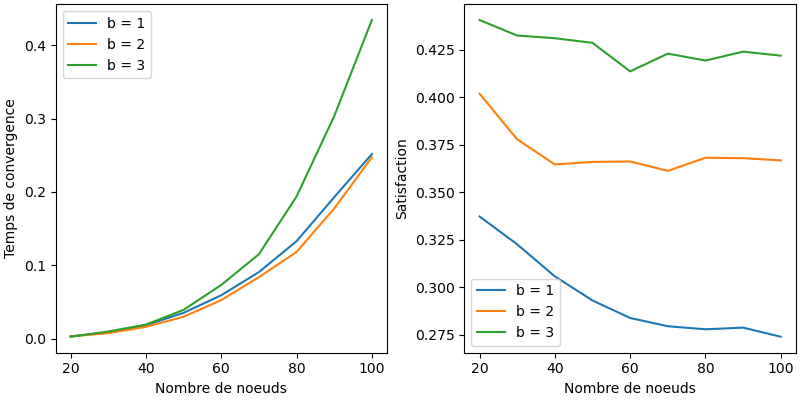
\includegraphics[width=0.9\linewidth]{chart_cyc_t_sat.png}
    \end{figure}
\end{frame}


% =================================================

\begin{frame}
    \frametitle{Conclusions et perspectives}

    \begin{itemize}
        \item Implémentation par couplages converge suffisamment rapidement
        \item La notion de satisfaction convient mieux que celle de couplage stable
        \item Perspectives: 
        \begin{itemize}
            \item Implémenter un algorithme réellement utilisé par les réseaux P2P $\rightarrow$ Comparaison
            \item Démontrer un facteur d'approximation pour l'algorithme de modification locale
        \end{itemize}
    \end{itemize}

\end{frame}

% =================================================

\begin{frame}
    \frametitle{Bibliographie}

    \begin{thebibliography}{9}

        \bibitem{cohen} B. Cohen,
        \textit{The BitTorrent Protocol Specification},
        BitTorrent.org: BEP 3, 2008


        \bibitem{lebedev}
        D. Lebedev et al.,
        \textit{On Using Matching Theory to Understand P2P Network Design},
        International Network Optimization Conference, 2007


        \bibitem{mathieu}
        F. Mathieu,
        \textit{Self-stabilization in preference-based systems},
        Discrete Applied Mathematics, 2007

        \bibitem{papa}
        G. Georgiadis, M. Papatriantafilou
        \textit{Adaptive distributed b-matching in overlays with preferences},
        International Symposium on Experimental Algorithms, 2012

    \end{thebibliography}

\end{frame}

% -------------------------------------------------
\end{document}